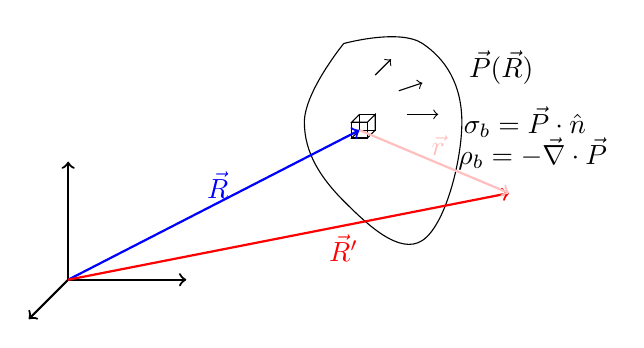
\begin{tikzpicture}

\draw  plot[smooth, tension=.7] coordinates {(2.5,3) (2,2) (2.5,1) (3.5,0.5) (4,2) (3.5,3) (2.5,3)};
\draw [<->, thick](-1,1.5) -- (-1,0) node (v1) {} -- (0.5,0);
\draw [->, thick] (v1.center) -- (-1.5,-0.5);
\draw  (2.6,2) node (v4) {} rectangle (2.8,1.8) node (v2) {};
\draw  (2.7,2.1) node (v5) {} rectangle (2.9,1.9) node (v3) {};
\draw (2.7,1.9) node (v6) {} -- (2.6,1.8) -- (v2.center) -- (v3.center) -- (2.9,2.1) -- (2.8,2) -- (v4.center) -- (v5.center);
\draw  [->, thick, blue](v1.center) -- (v6.center);
\draw  [->, thick, red](v1.center) -- (4.6,1.1) node (v7) {};
\draw  [->, thick, pink](v6.center) -- (v7.center);
\node at (0.9,1.2) [blue] {$\vec{R}$};
\node at (3.7,1.7) [pink]{$\vec{r}$};
\node at (2.5,0.4) [red]{$\vec{R}'$};
\draw [->] (2.9,2.6) -- (3.1,2.8);
\draw [->]  (3.2,2.4) -- (3.5,2.5);
\draw  [->] (3.3,2.1) -- (3.7,2.1);
\node at (4.5,2.7) {$\vec{P}(\vec{R})$};
\node at (4.8,2) {$\sigma_b=\vec{P}\cdot \hat{n}$};
\node at (4.9,1.6) {$\rho_b=-\vec{\nabla}\cdot\vec{P}$};
\end{tikzpicture}